\documentclass[12pt]{article}
\usepackage[usenames]{color} %used for font color
\usepackage{amsmath, amssymb, amsthm}
\usepackage{wasysym}
\usepackage[utf8]{inputenc} %useful to type directly diacritic characters
\usepackage{graphicx}
\usepackage [english]{babel}
\usepackage [autostyle, english = american]{csquotes}
\MakeOuterQuote{"}
\graphicspath{ {./} }
\newcommand{\Z}{\mathbb{Z}}
\newcommand{\N}{\mathbb{N}}
\newcommand{\R}{\mathbb{R}}
\newcommand{\Q}{\mathbb{Q}}
\newcommand{\prob}{\mathbb{P}}
\newcommand{\degrees}{^{\circ}}


\author{Tianshuang (Ethan) Qiu}
\begin{document}
\title{Math 74, Week 4}
\maketitle

\section{Lec Mon, 1c}
\subsection{a}
Since each term is the product of $x^a, y^b, z^c$, and $a+b+c = 2020$, we can simplify this problem into dogs and biscuits. $\binom{2020+3-1}{3-1} = \binom{2022}{2}$

\subsection{b}
Before combining, we expand each term by picking one variable from each of the 2020 $(x+y+z)$ multiplied together. So we have $3^2020$.

\subsection{c}
We can reach the same result by subtracting the amount where there is only $x$, or only $y$, or only $z$, or $xy$, $xz$, $yz$.
\newline
For the first three, there is only 1 way for that to happen since that variable has to be raised to 2020. For $xz$, we have $a+b = 2020$, feeding 2018 biscuits to 2 dogs. We need to subtract 2 since we have already counted having only one term. Therefore $\binom{2018+2-1}{2-1} = 2019$.
\newline
Adding them together we have $1 \times 3 + 2019 \times 3 = 6060$
\newpage


\section{Dis Mon, 1a}
LHS is the amount of ways to choose a team with $k$ people and a captain from a group with $n$ people. It chooses the team first: $\binom{n}{k}$. Then from that team we choose a captain with $k$ ways to do it.
\newline
RHS calculates the amount of ways to choose a captain first: $n$, then the rest of the team: $\binom{n-1}{k-1}$. Both sides calculate the same thing. Therefore LHS = RHS.
\newline
Q.E.D.

\section{Dis Mon, 4}
$$x+\frac{1}{x}=7$$
$$(x+\frac{1}{x})^2=49$$
$$x^2+\frac{1}{x^2}+2=49$$
$$x^2+\frac{1}{x^2}=47$$
\newpage

\section{Lec Wed, 1a}

\begin{figure}[h]
    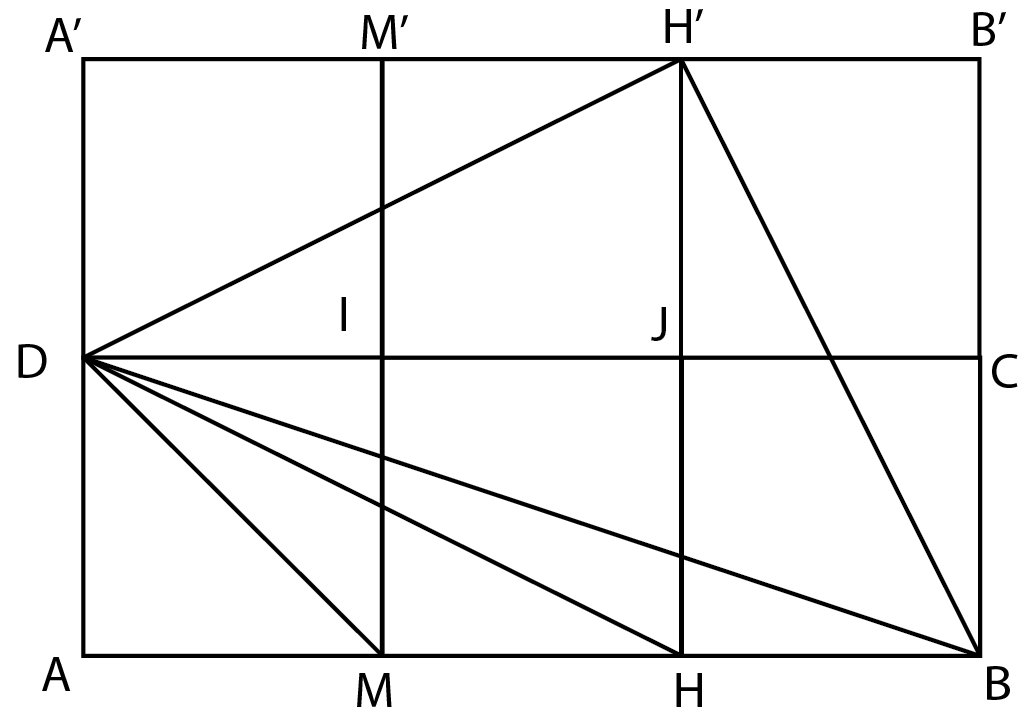
\includegraphics{GRAPH1}
\end{figure}
The sum of these angles is 90$\degrees$.
\newline
Proof: We attempt to move all three angles to $\angle HBC$, since a square has 4 right angles, we can see that $\angle HBC = 90\degrees$.
\newline
We construct a row of 3 identical squares with $A'M' = AM, M'H' = MH, etc$, and connect $DH', H'B$
\newline
Consider $\triangle DAM$, it is a right isosceles triangle, since it is in a square ($DA = AM, DA \perp AM$). Now consider $\triangle DA'H', \triangle H'B'B$. Since all the squares have the same side length, we have $DA' = H'B', A'H'=B'B$. Furthermore, since these are all squares, we have $\angle DA'H' = \angle H'B'B = 90\degrees$.
\newline
Therefore $\triangle DA'H' \cong \triangle H'B'B$ by SAS property. $DH' = H'B, \angle H'B'B = \angle DH'A$. Since the sum of the three angles in a triangle is $180\degrees$ and $\angle H'B'B = DA'H' = 90\degrees$, we can see that $\angle B'H'B + \angle AH'D = 90\degrees$. Finally, since M'H'B' forms a line $\angle M'H'B' = 180 \degrees$, we have $\angle DH'B = \angle DAM = 90 \degrees$.
\newline
Now we have $\triangle DH'B \sim \triangle DAM$ by RAR property for similarity, therefore $\angle AMD = \angle H'BD$.
\newline
By essentially the same logic as $\triangle DA'H' \cong \triangle H'B'B$, we can prove that $\triangle DAH \cong \triangle H'B'B$, so $\angle DHA = \angle B'BH$.
\newline
We have proven that $\angle AMD = \angle H'BD$, $\angle DHA = \angle B'BH$. Since the sum these two and $\angle DBA$ is a right angle, we have proven our claim.
\newpage

\section{Lec Wed, 1b}
\begin{figure}[h]
    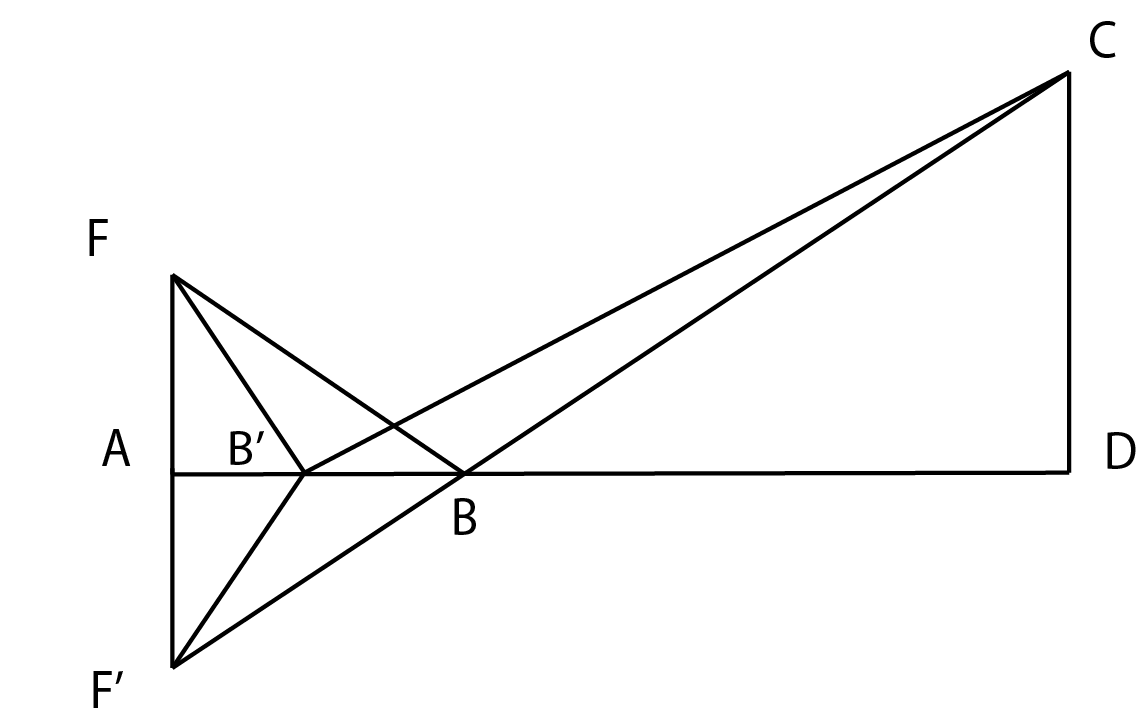
\includegraphics[width = 100mm]{GRAPH2.png}
\end{figure}
We reflect F over $AD$ to $F'$, and connect $F'C$. Now we first show that B is the optimal point.
\newline
By the definiton of reflection, we can see that if we were to reflect $F'$ back over $AD$ it will overlap with our original point. This "overlap" causes all three vertices of $\triangle ABF$ to overlap with those of $\triangle ABF'$. By Euclid's definition they are congruent.
\newline
Consider a point on $AD$ that is not $B: B'$. By similar reasoning we can also show that $\triangle AB'F \cong \triangle AB'F'$.
\newline
From these congruencies we see that $B'F = B'F', BF = BF'$. The farmers route can then be converted into $F'B+B'C$ and $F'B + BC$. Furthermore, since F'B'C forms a triangle, we have $F'B+B'C > F'B + BC$ by the triangle inequality, thus proving that B gives the shortest route to the cow.
\newline
Since $FF' \perp AD$ and $CD \perp AD$, we have $FF' \parallel CD$. By the property of alternate interior angles, $\angle FF'C = \angle F'CD$.
\newline
$\angle ABF' + \angle ABC = 180 \degrees$ since F'C is a line. By the same logic, $\angle CBD + \angle ABC  = 180 \degrees$. Therefore $\angle ABF' = DBC$. We have now shown $\triangle ABF' \sim \triangle CBD$ by AAA property.
\newline
$AF = AF' = 2$. Let $AB = x$, $BD$ would then equal $4-x$. By property of similarity we have $\frac{CD}{F'A} = \frac{DB}{AB}$
$$\frac{6}{2} = \frac{4-x}{x}$$
Solving the above equation yields $x=1$.
\newpage


\section{Wed Lec, 2b}
\begin{figure}[h]
    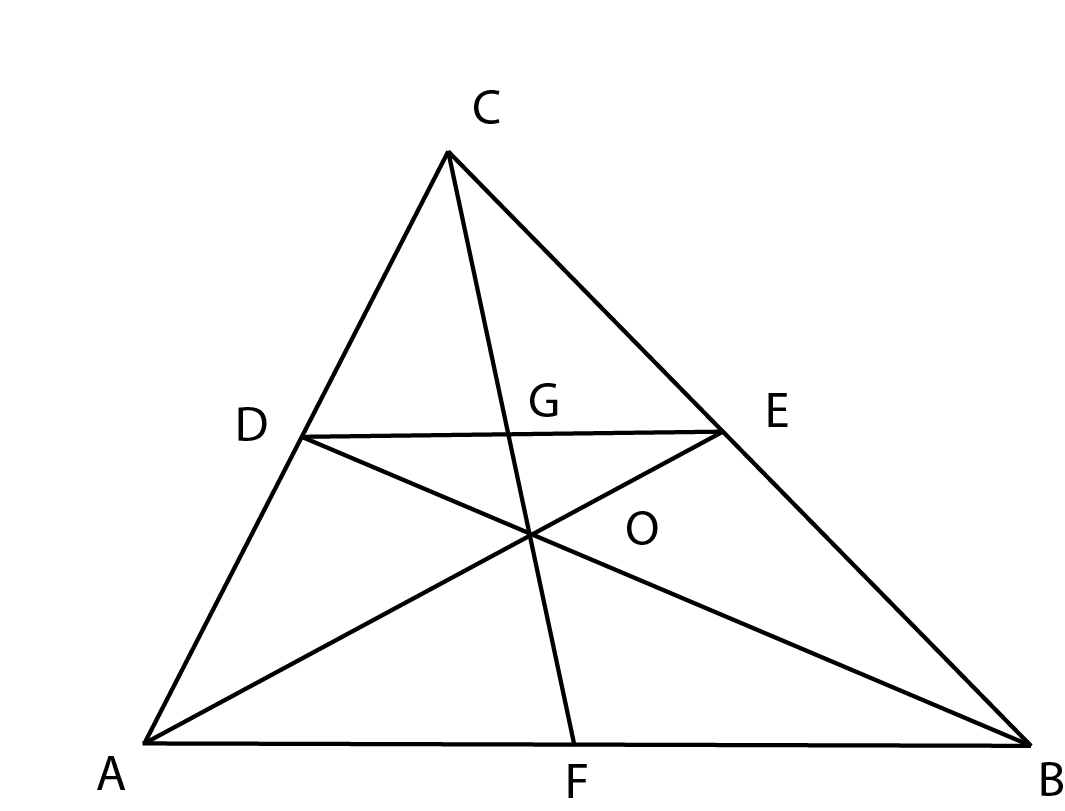
\includegraphics[width = 100mm]{GRAPH3.png}
\end{figure}
Let $AD = CD, CE = EB$, the two segments intersect at O. Connect $BD$, $AE$, $DE$, $CO$, and extend $CO$ to intersect $AB$ at $F$.
\newline
This assumes that 2a ($DE \parallel AB$, $DE = 0.5AB$) has already been proven.
\newline
Since $DE \parallel AB$, the alternate interior angles are equal, $\angle EDB = \angle DBA$, $\angle DEA = EAB$. Since the sum of all the angles of a triangle is $180 \degrees$, the third angle must also be the same. Therefore $\triangle DEO \sim \triangle BAO$ by AAA similarity.
\newline
Because $DE = 0.5AB$, $DO = 0.5BO, EO = 0.5 AO$.
\newline
Using $DE \parallel AB$ again, we can see that $\angle EGF = \angle AFG$. By the same reasoning as above we can see that $\triangle GOE \sim \triangle FOA$ by AAA similarity. Therefore $$\frac{GE}{AF} = \frac{EO}{OA} = \frac{1}{2}$$.
Since $DE \parallel AB$, we can show that $\angle CGE = \angle CFB$, $\angle CEG = \angle CBF$ due to the corresponding angles being equal. $\triangle CGE \sim \triangle CFB$ by AAA similarity. $GE = 0.5FB$
\newline
Since $GE = \frac{1}{2}FB = \frac{1}{2}AF$, $AF = FB$. Therefore all three medians intersect at point $O$.
\newpage


\section{Dis Wed, 1a}
\begin{figure}[h]
    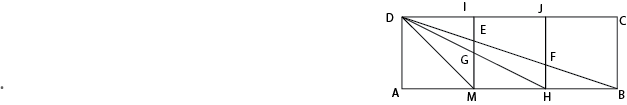
\includegraphics[width = 100mm]{GRAPH4.png}
\end{figure}
Connect $JB$.
\newline
We first prove a congruency between two right triangles. Since these are all squares we have $DA = AM = BC = CJ$, and $\angle DAM = \angle BCJ = 90 \degrees$. Therefore $\triangle DAM \cong JCB$ by SAS congruency.
\newline
Therefore $\angle DMA = \angle CBJ = \angle BCJ = 45 \degrees$ due to the triangle being isosceles and right. Let $DA$ have length $x$, then $DM$ would have length $\sqrt 2$. Since $\angle DMA = 45 \degrees$, its compliment $\angle DMH = 135 \degrees$. Similarly, $\angle BJC$'s compliment $\angle BJD = 135 \degrees$. $DJ$ has length 2x, and $JB$ has length $\sqrt 2$.
\newline
$\frac{MH}{JB} = \frac{DM}{DJ}$, and since the $\angle DMH = \angle BJD = 135 \degrees$, $\triangle DMH \sim \triangle DJB$, and $\angle DHM = \angle JBD$.
\newline
Thus we have moved all three angles into the right angle $\angle HBC$, proving that the sum of these three angles is $90 \degrees$. Q.E.D.
\newpage

\section{Wed Dis, 3b}
\begin{figure}[h]
    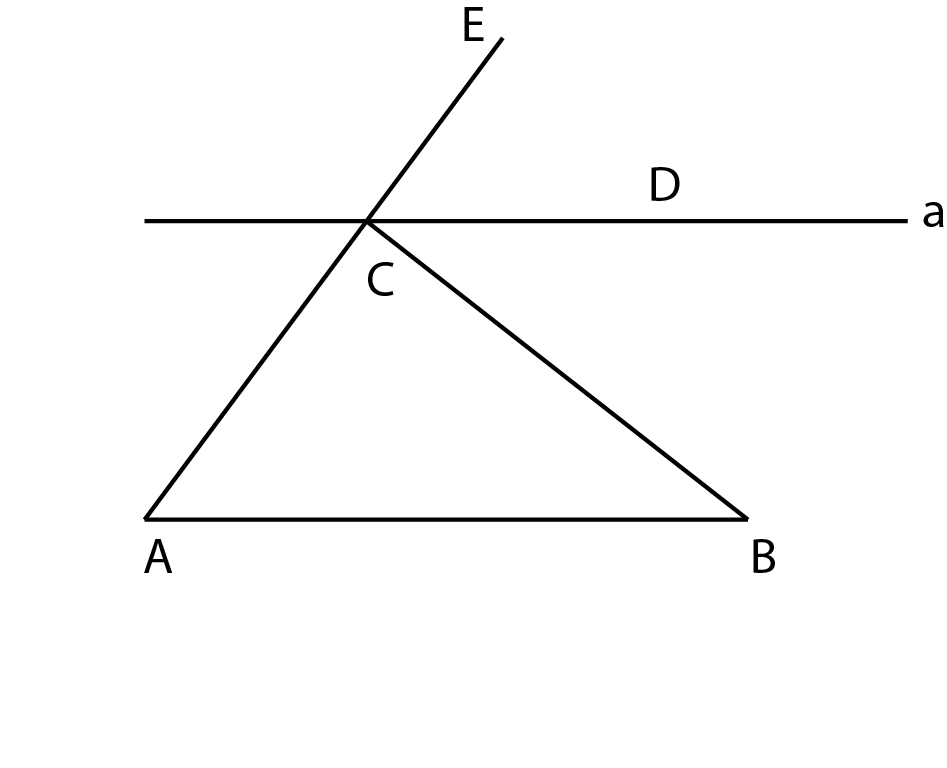
\includegraphics[width = 100mm]{GRAPH6.png}
\end{figure}
Let $\triangle ABC$ be an arbitrary triangle, extend AC to E, construct $a \parallel AB$.
\newline
For this proof I need the axiom that a straight line is $180 \degrees$, and that the corresponding angles and alternate interior angles between two parallel lines are equal.
\newline
Since $a \parallel AB$, we have $\angle BAC = \angle DCE$, and $\angle ABC = \angle BCD$. Since the three angles form $\angle ACE$, which is a straight line, the 3 angles add up to $180 \degrees$.
\newpage


\section{Fri Lec, 3}
If the 5th postulate was indeed redundant (provable from others), then the 4 postulates alone must always define the Euclidean space, and that there should be no other spaces that could follow the first 4 postulates but not the fifth.
\newline
Hyperbolic geometry satisfies the first 4 with its own definitions of lines, circles, and right angles. The resulting space does not follow Euclid's 5th postulate: two lines whose sum of the inner angles on one side is less than $180 \degrees$ can still curve away from each other and never intersect.
\newline
This shows that we need Euclid's 5th postulate to properly define a Euclidean space.
\newpage


\section{Fri Lec, 4b}
Let us label "There is at most 1 parallel line to a given line $l$ through a given point $P$" "Statement A", and "two lines that are parallel to  the same line are also parallel to eachother" "Statement B".
\newline
For this problem we need to prove that $A \iff B$. We will begin by proving $A \implies B$.
\newline
\begin{figure}[h]
    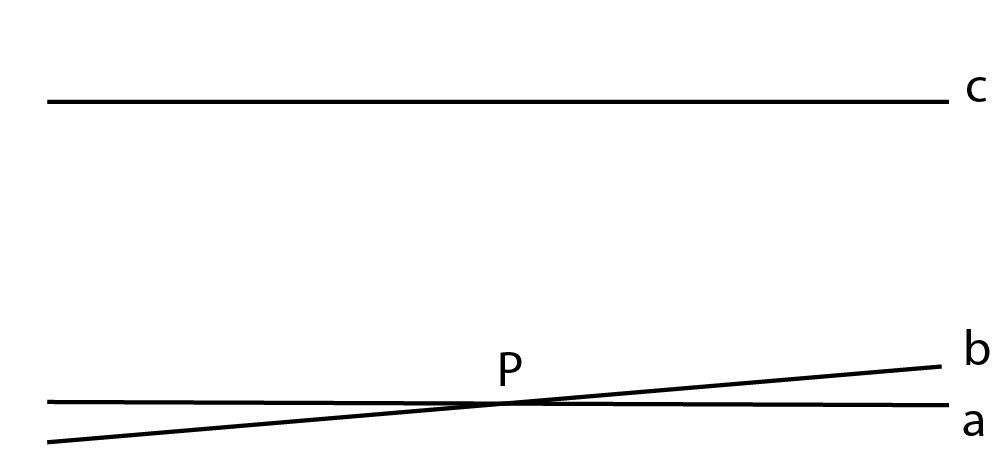
\includegraphics[width = 100mm]{GRAPH5.png}
\end{figure}
\paragraph{1}
Assume that statement B is false, so the two lines are not parallel to each other. Then let $a \parallel c, b \parallel c$, and $a, c$ intersect at point $P$. Then at $P$, there are two different lines that are both parallel to $c$. \lightning
\newline
Therefore our initial assumption is incorrect, statement B is true.
\paragraph{2}
Now we try to prove that $B \implies A$. Assume that statement A is false, so there are at least 2 different lines that go through that point. Then let $a \parallel c, b \parallel c$, $a,b$ go through the same point $P$.
Then by statement B, $a \parallel b$, but $a, b$ both contain $P$, so they have to be the same line. \lightning
\newline
Therefore there exists at most one line through $P$ parallel to $c$.

\end{document}
